

%---------------------导言区---------------------------%
\documentclass[10pt,a4paper,twocolumn,twoside,UTF8]{ctexart}
	%10pt:正文字体为10pt,可以缺省;各层级字体大小会根据正文字体自动调整
	%a4paper:纸张大小a4;
	%twocolumn:双栏排版;
	%twoside:排版上分奇偶页,一般也就是有双面打印的需求;
	%UTF8:中文要求
\usepackage{geometry}%用于设置上下左右页边距
	%左右边距一样: 不考虑装订和翻页的需要.实验室网站上的示例论文格式报告就是这样。
	\geometry{left=2cm,right=2cm,top=2.5cm,bottom=4cm}
	%实际上,一般需要考虑到双面打印、装订和翻页的需要,需要区分奇偶页。奇偶页的页边距需要分开设置。奇数页左边距较宽,偶数页左边距较窄。
\usepackage{xeCJK,amsmath,paralist,enumerate,booktabs,multirow,graphicx,float,subfig,setspace,listings}
	%xeCJK:中文字体(如楷体,作者和机构需要用到)的设置
	%amsmath:数学公式
	%paralist,enumerate:自定义项目符号
	%booktabs:三线图,论文常用的表格风格
	%multirow:复杂表格
	%graphicx,float: 插入图片
	%subfig:并排排版图片以及强制图表显示在“这里”[H]
	%setspace:设置行间距等功能
	\setlength{\parindent}{2em}%正文首行缩进两个汉字
	%listings:用于排版各种代码;比如matlab的代码
	\lstset{language=Matlab}%matlab代码
	%代码环境的使用可以参考完整实验报告模板

\setCJKmainfont{FZShuSong-Z01S}[ItalicFont=FZKai-Z03S, BoldFont=FZHei-B01S]
%中文字体设置:使用开源字体方正书宋,方正楷体和方正黑体

\usepackage{titlesec}
	%改变section、subsection里面字体的样式。中文黑体,英文TNR。
	\newfontfamily\sectionef{Times New Roman}
	\setCJKfamilyfont{FZHeiTi}{FZHei-B01S}
	\newcommand{\sectioncf}{\CJKfamily{FZHeiTi}}
	\titleformat*{\section}{\large\bfseries\sectioncf\sectionef}
	\titleformat*{\subsection}{\normalsize\bfseries\sectioncf\sectionef}


\usepackage{fancyhdr}
	%fancyhdr:一个很强大的宏包,用于自定义设计页面风格并命名以供调用。



%%begin----------设置首页和正文不同的页眉页脚----------------%%

\usepackage{ifthen}%这个宏包提供逻辑判断命令
\newboolean{first}%引入布尔变量
\setboolean{first}{true}%将布尔变量设置为true
\pagestyle{fancy}

	%%% Step1 定义正文的页面风格
	%E表示偶数页,O表示奇数页;R、L、C代表文字居右、居左、居中排版
	%页码:保证在外侧, 奇数页分布在右边,偶数页分布在左边
	%页眉中间的内容也因奇偶页而不同
	%实验名称根据实际情况修改
	\fancypagestyle{maincontent}{
		\fancyhf{}  %清空页眉页脚设置
		\fancyhead[EL, OR]{\thepage}
		\fancyhead[EC]{Pregel:一个大规模图计算系统}
		\fancyhead[OC]{大\quad 数\quad 据\quad 技\quad 术\quad 报\quad 告}
		\renewcommand\headrulewidth{0pt}
	}

	%%% Step2 定义首页的页面风格
	%页眉中间的双行文字,大小和字间距需要微调
	%左右的内容是年月,可以自己修改寻找自动获取的方法
	\usepackage{datetime}
		%\shortmonthname可以获取英文月份缩写
	\fancypagestyle{firstpage}{
		\setboolean{first}{false}%firstpage出现,则将first重置为false
		\fancyhf{}  %清空页眉页脚设置
		\fancyhead[L]{\the\year 年\the\month 月}
		\fancyhead[R]{\shortmonthname[\the\month], \the\year}
		\fancyhead[C]{
		          \large{大\quad 数\quad 据\quad 技\quad 术\quad 报\quad 告}\\
		          \normalsize{BIG DATA TECHNOLOGY REPORT}
		          }
	}

	%%% Step3 页眉线的设置:用布尔变量区分首页和正文
	\newcommand{\makefirstpageheadrule}{%定义首页页眉线-双线绘制命令
		\makebox[0pt][l]{\rule[0.55\baselineskip]{\headwidth}{0.2pt}}%上0.5pt,下0.2pt
		\rule[0.7\baselineskip]{\headwidth}{0.5pt}
	}

	\newcommand{\makeheadrule}{%定义正文页页眉线绘制命令,单线
		\rule[0.7\baselineskip]{\headwidth}{0.75pt}
	}

	%根据布尔变量first为true或false分别执行不同的页眉线绘制命令
	\renewcommand{\headrule}{%重定义headrule命令
		\ifthenelse{\boolean{first}}{\makeheadrule}
		{\makefirstpageheadrule}
	}



%%end--------------设置首页和正文不同的页眉页脚-----------%%



%%begin-----------------参考文献-----------------------%%

\usepackage{hyperref}%超链接
\usepackage[hyperref=true,backend=biber,bibstyle=gb7714-2015,citestyle=numeric-comp,sorting=none,backref=true]{biblatex}
	%hyperref=true和backref=true表示为各个参考文献的引用处、及定理、定义、例子等的引用处都添加上超链接;
	%backend=biber:后端处理的程序为biber.exe
	%bibstyle:参考文献风格;每个期刊、组织要求不同
		%gb7714-2015是目前国内期刊通用的风格,称为gb标准风格
	%citestyle:引用风格;每个期刊、组织要求不同
	%sorting=none:按照参考文献在论文中出现的先后顺序排序。
	%**编译:biblatex与biber命令配合使用。xelatex-biber-xelatex-xelatex
\addbibresource{book.bib}
	%这里写上.bib文件的相对地址
	%每次实验引用的页数不同,需要手动改变

%%end-------------------参考文献-----------------------%%




%%%%%%%%%%%%%%%%%%%%%%%%%%%%%%%%%%%%%%%%%%%%%%%%%%%%%%%%%%
%%%%%%%%%%%%%%%%%%%%%%%%%正文开始%%%%%%%%%%%%%%%%%%%%%%%%%%
%%%%%%%%%%%%%%%%%%%%%%%%%%%%%%%%%%%%%%%%%%%%%%%%%%%%%%%%%%

\begin{document}


%%begin-------------------中文摘要-----------------------%%
\title{\LARGE\textbf{Pregel:一个大规模图计算系统}}
\author{\large\textit{李妍妍}$^{1}$\\ \normalsize{(1 \textit{广州大学 {} 计算机科学与网络工程学院,广东{} 广州 }510000)}}
\date{}%不显示日期

\twocolumn[
	%twocolumn: 双栏article下的单栏摘要
	\begin{@twocolumnfalse}
	\maketitle  %标题和作者
  	\renewcommand{\abstractname} {} %不显示摘要名字
	\begin{abstract}
	\vspace{-3em}
	%vspace:调整垂直空白,可以自己调整;缩小abstract和center(以及maketitle)的间距
	%\noindent %备用:摘要无缩进
	{\bf 摘{} 要:}
	{\small 在许多实际计算问题中,大数据都是以大规模图或网络的形式呈现。而传统的图计算存在着诸如内存访问局部性等问题。Google在2010年提出了一种适用于此任务的计算模型,即Pregel。Pregel是一种基于BSP模型实现的并行图处理系统。在该系统中,程序是一系列的迭代,每个顶点都可以接收在前一个迭代中发送的消息,然后发送消息给其他顶点,并修改自己的状态和其输出边的状态,或改变图拓扑结构。这种以顶点为中心的方法足够灵活,可以表达一组广泛的算法。Pregel就搭建了一套可扩展的、有容错机制的平台,该平台提供了一套非常灵活的API,可以描述各种各样的图计算。本文详细的介绍了并行计算模型BSP和Pregel的基本原理及其基础架构。}
	\par%空的新行的高度。
	\textbf{关键词}:大数据,分布式计算,图算法,Pregel
	\vspace{2em}
	\end{abstract}
	\end{@twocolumnfalse}
]

%%end-------------------中文摘要-----------------------%%

\thispagestyle{firstpage}%首页页面风格:firstpage
\pagestyle{maincontent}%第二页之后的页面风格:maincontent

%%begin----------------层级结构------------------------%%

%重点1:知道每一个层级的样式和怎么和后面的正文接上
%重点2:掌握各种换段的方法
%重点3:自定义的项目符号(宏包enumerate的用法)

\section{引 \quad 言}
	%%section:第一级,节	,1
互联网使网格化图形成为分析和研究的热门对象。例如运输路线、报纸文章的相似性、疾病爆发的路径、或发表的科学作品之间的引用关系。常用的算法包括最短路径计算、不同类型的聚类算法,还有许多具有实用价值的图计算问题,如最小割和连通分量等。高效处理这些大型图形常常是具有挑战性。传统的图算法通常表现出较差的内存访问局域性,每个顶点的工作量很少,并且在执行过程中并行度不断变化,分布在多台机器上加剧了局部性问题,并增加了机器在计算过程中失败的概率。Pregel 是 Google 自 2009 年开始对外公开的图计算算法和系统, 主要用于解决无法在单机环境下计算的大规模图论计算问题。与其说 Pregel 是图计算的算法, 不如说它是一系列算法、模型和系统设计组合在一起形成的一套图模型处理方案。图计算的实际应用非常广泛,因此自 Pregel 公开之后,一些开源的方案也被实现出来, 比如说来自 Spark 的 GraphX 就实现了 PregelAPI。 值得注意的是,Pregel 作为一个近十年前起就为人所知的算法,虽然新近也已经提出了不少增强和改进的技术, 但在现实场景下仍然是很有生命力的。\par
	%%section后面的正文:自动换段,正常缩进
	%%PS:这里出现了引用。一般就是做个样子,在引言引一下参考文献就好了。不引用后面的参考文献打印不出来。\cite{shenhan2015}
	%%自然换段:\par
目前的图计算模型基本上都遵循BSP计算模式。在详细介绍Pregel模型之前,我们先简单了解一下BSP模式的相关概念。

\newpage
%换一栏,而不是换一页。换一页用\clearpage
\section{BSP模式}
BSP(Bulk Synchronous Parallel,整体同步并行)是一种并行计算模式,由英国计算机科学家Viliant在上世纪80年代提出。BSP计算模式如图1所示:
%%% 1 不跨栏单幅图
	% 图片的大小需要细细得调。需要掌握latex里面的长度单位和限制大小方法。
	\begin{figure}[htbp]
		\centering
		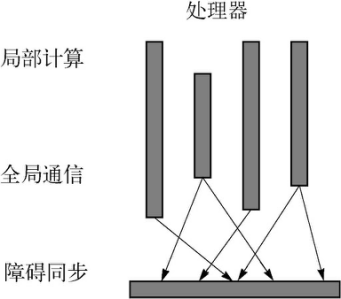
\includegraphics[width=0.4\textwidth]{img//pic1.png}
			%textwidth:正文宽度。双栏,则将两栏正文宽度相加。
		\caption{BSP计算模式图}
		\label{pic1}
	\end{figure}
	
	作为计算机语言和体系结构之间的桥梁,BSP使用下面三个参数(或属性)来描述的分布存储的多处理器模型:处理器/储器模块;执行以时间间隔L为周期的所谓路障同步器和储器模块对之间点到点传递消息的选路器。\par
所以BSP模型将并行机的特性抽象为三个定量参数p、g、L,分别对应于处理器数、选路器吞吐率(亦称带宽因子)、全局同步之间的时间间隔。

	\subsection{BSP模型中的计算行为}
	在BSP模型中,计算过程是由一系列用全局同步分开的周期为L的超级步(supersteps)所组成的。一个抽象的程序由分布在n个处理器上的p个进程或线程组成,并且被分为superstep。在各superstep中,每个处理器均执行局部计算,并通过选路器接收和发送消息;然后做一全局检查,以确定该超级步是否已由所有的处理器完成:若是,则前进到下一超级步,否则下一个L周期被分配给未曾完成的超级步。BSP计算模式中以下几个概念需要了解一下:\par
	%%paragraph后面的换段方法
	 {(1)Processors:}~ 并行计算进程,它对应到集群中的多个结点,每个结点可以有多个Processor。\par
	{(2)LocalComputation:}~ 单个Processor的计算,每个Processor都会切分一些结点作计算。\par
	{(3)Communication:}~ Processor之间的通信。接触的图计算往往需要做些递归或是使用全局变量,在BSP模型中,对图结点的访问分布到了不同的Processor中,并且哪怕是具有局部聚类特点的结点也未必会分布到同一Processor上,所有需要用到的数据都需要通过Processor之间的消息传递来实现同步。\par
	{(4)BarrierSynchronization:}~ 栅栏同步。每一次同步也是一个超步的完成和下一个超步的开始。\par
       {(5)Superstep:}~ 超步,这是BSP的一次计算迭代,拿图的广度优先遍历来举例,从起始结点每往前步进一层对应一个超步。\par
       任务结束,一个作业可以选出一个Proceessor作为Master,每个Processor每完成一个Superstep都向Master反馈完成情况,Master在N个Superstep之后发现所有Processor都没有计算可做了,便通知所有Processor结束并退出任务。
      
		% ~是一个控制符号,不会真的输出~,而是空一格。
	%\newline %换行,强制换行之后需要手动缩进,用命令\indent
	

	\subsection{BSP成本分析(Computational analysis)}
	考虑一个由S超步骤组成的BSP程序。那么,超步骤i的执行时间为:
		%一般来说都需要标号
		\begin{equation}
		 T_{super} = \substack{\max\\processes} +\max gh_i + L  
		\end{equation}
	其中, wi是进程 i(process i)的局部计算函数, hi是进程 i发送或接收的最大数据包,g是带宽的倒数(时间步/数据包), L是路障同步时间(注意我们不考虑I/O的传送时间)。所以,在BSP计算中,如果使用S个超级步,则总运行时间为:
	
		\begin{equation}
		T_{BSP} = \sum\limits_{i = 0}^{S-1} w_i  + g\sum\limits_{i = 0}^{S-1}h_i + SL  
		\end{equation}
	
	$w_i$和$h_i$分别被称为超步骤的深度和程序的深度

%%end------------------层级结构------------------------%%

%%begin------------------插入图表------------------------%%

\section{Pregel的计算模型}
	在BSP模式的基础上,我们详细解释一下Pregel模型的原理。Pregel在概念模型上遵循BSP模式。整个计算过程由若干顺序运行的超级步(Super Step)组成,系统从一个“超级步”迈向下一个“超级步”,直到达到算法的终止条件。一个典型的Pregel计算过程如下:
%%% 1 不跨栏单幅图
	% 图片的大小需要细细得调。需要掌握latex里面的长度单位和限制大小方法。
	\begin{figure}[htbp]
		\centering
		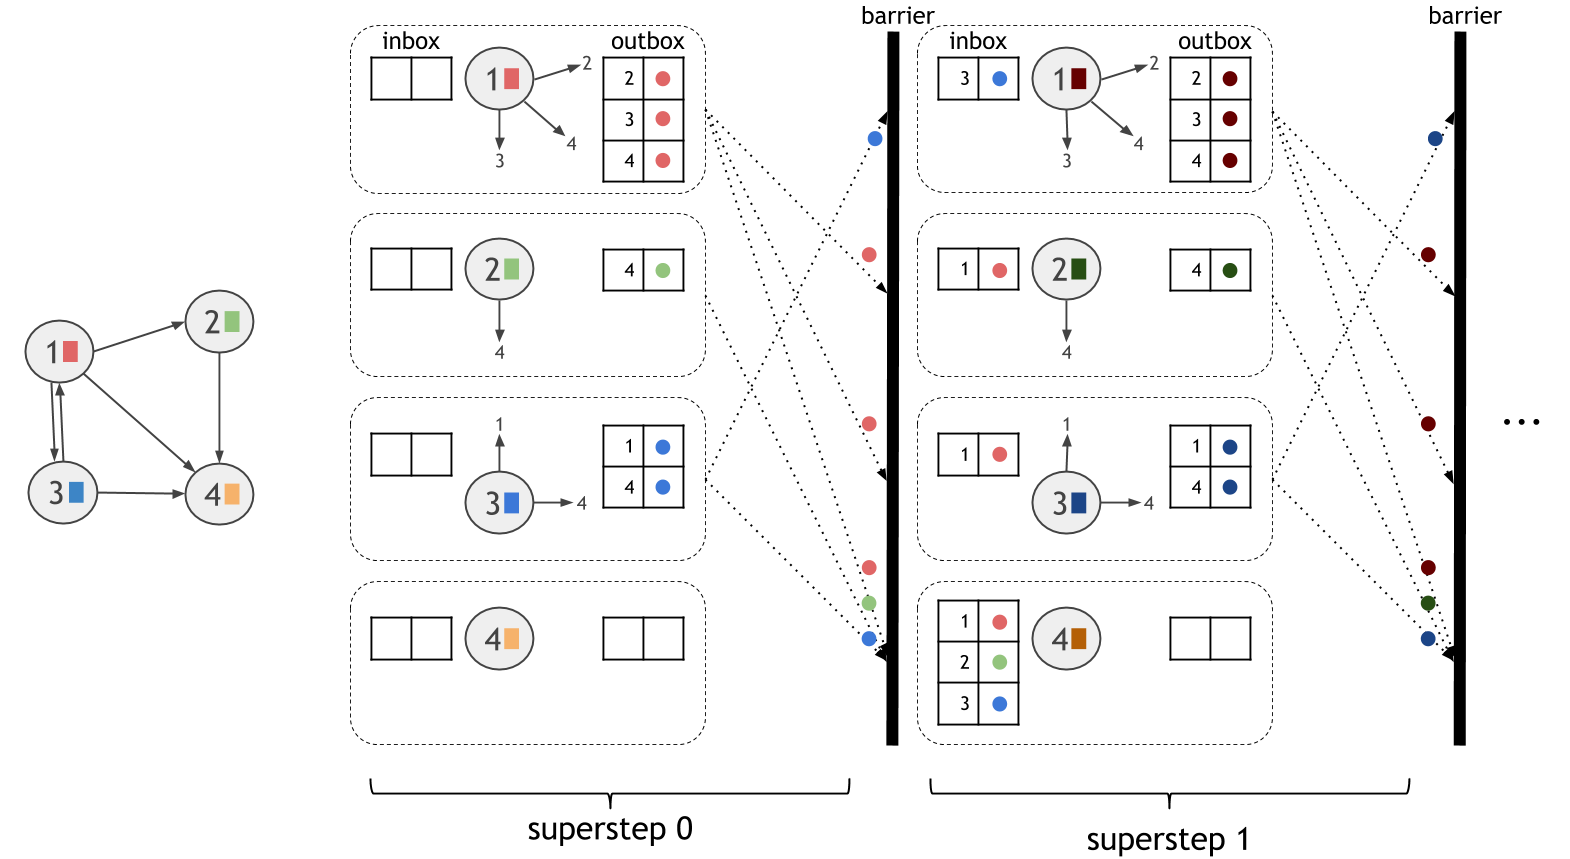
\includegraphics[width=0.5\textwidth]{img//pic2.png}
			%textwidth:正文宽度。双栏,则将两栏正文宽度相加。
		\caption{Pregel计算过程}
		\label{pic2}
	\end{figure}
	其计算过程遵循下面的步骤:
	\begin{enumerate}[(1)]
		\item 读取图数据并对图初始化;
		\item 当图被初始化完毕,执行一系列的超步(SuperStep)直到整个计算结束,这些SuperStep之间通过一些全局的同步点分隔;
	 	\item 输出计算结果。
	\end{enumerate}
	
	在每个SuperStep中,顶点上的计算都是并行的,每个顶点执行相同的用于表达指定逻辑的用户自定义函数。每个顶点都可以需修改自身以及出边的状态,接收前一个SuperStep发送给它的消息,并将计算的结果或信息发送给其他顶点,这些信息会在下一个SuperStep中被目标顶点接收。边在这种计算模式中并不是核心对象,只用于表明消息传递的方向,没有相应的计算运行在其上。
		
	\subsection{Pregel模型状态机}
	算法结束的时机取决于所有的顶点是否均已经达到halt状态。整个状态转换如下图所示:
	\begin{figure}[htbp]
		\centering
		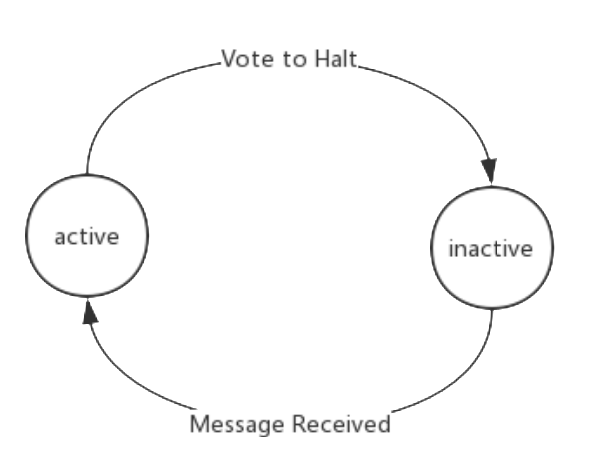
\includegraphics[width=0.4\textwidth]{img//pic3.png}
			%textwidth:正文宽度。双栏,则将两栏正文宽度相加。
		\caption{Pregel状态转换图}
		\label{pic3}
	\end{figure}
	
	 图3中,首先在刚开始的时候,所有的顶点都处于active状态,所有的active顶点都会参与到SuperStep中的相应计算。顶点通过将其自身的status设置成inactive来表示它已不再active,以此表明在下一次的SuperStep中,该顶点不再需要执行相应的计算。除非该顶点接收到其他顶点传送的消息,否则Pregel框架不会再接下来的SuperStep中执行该顶点的计算。如果顶点在接收到消息后进入active状态,那么在随后的计算中该顶点必须显式的deactive。整个计算在所有顶点都达到inactive状态,并且没有消息传送时结束。
	 \subsection{Pregel模型示例}
	接下来展示一个以Pregel计算最大值的例子。假设图中存在A/B/C/D四个顶点,其中每个顶点的数据表示当前顶点的值。在计算的每个SuperStep中),每个顶点将接收其他顶点传过来的值(初始SuperStep除外),并判断当前顶点的值是否小于传递过来的值。若小于,更新当前顶点的值,并将该顶点状态设置为active状态,同时将当前顶点的最新值传递出去;若不小于,则什么都不做,并将当前顶点的状态设置为inactive。直到所有的顶点状态均变成inactive,计算结束。整个过程入下图所示:
	
	\begin{figure}[htbp]
		\centering
		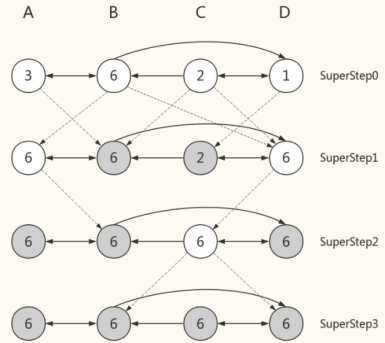
\includegraphics[width=0.4\textwidth]{img//pic4.png}
			%textwidth:正文宽度。双栏,则将两栏正文宽度相加。
		\caption{Pregel模型示例图}
		\label{pic4}
	\end{figure}
	
	以图4为例,我们详细介绍一下Pregel模型的执行过程。\par	
	\begin{itemize}
		\item[$\bullet$] SuperStep0:初始SuperStep,不接收信息,只负责将当前顶点的值传递出去,并设置所有顶点状态为active。
		\item[$\bullet$] SuperStep1: 顶点A接收的信息为6,将当前顶点的值设置为6,状态设置为active,并将6作为消息发送给顶点B(顶点B下一轮迭代的时候会收到,当前轮次并不会收到);顶点B接收的信息为3和2,均小于当前顶点值6,不更新当前顶点值,并将顶点的状态设置为inactive;顶点C接收的信息为1,小于当前顶点值2,不更新当前顶点值,并将顶点的状态设置为inactive;顶点D接收信息为2和6,将当前顶点的值更新为6,状态设置为active,并将6作为消息发送给顶点C;
		\item[$\bullet$]SuperStep2:顶点A未接收到信息,且状态为inactive,什么都不做;顶点B接收到顶点A上一个轮次发送的消息,由于当前顶点值为6,不小于接收到的消息6,因此不更新当前顶点值,并将顶点的状态设置为inactive;顶点C接收到的消息为6,当前顶点值为2,将当前顶点的值更新为6,状态设置为active,并将6作为消息发送给顶点B和D;顶点D未接收到信息,且状态为inactive,什么都不做;
		\item[$\bullet$]SuperStep3:顶点A未接收到信息,且状态为inactive,什么都不做;顶点B接收到顶点C上一个轮次发送的消息,由于当前顶点值为6,不小于接收到的消息6,因此不更新当前顶点值,并将顶点的状态设置为inactive;顶点C未接收到任何信息,因此将状态设置为inactive;顶点D接收到顶点C上一个轮次发送的消息,由于当前顶点值为6,不小于接收到的消息6,因此不更新当前顶点值,并将顶点的状态设置为inactive;
	\end{itemize}
	
	顶点的状态均为inactive,迭代停止,输出结果。
	
	\subsection{Pregel的一些应用}
	\subsubsection{PageRank}
	在实现PageRank时,首先,我们实现PageRankVertex类,继承Vertex. 顶点用一个double 来存储当前的PageRank值。因为边不存储数据,边的类型是void。我们设置Graph在超级步0初始化,每个顶点的值是1/NumVertices()。
	\begin{figure}[htbp]
		\centering
		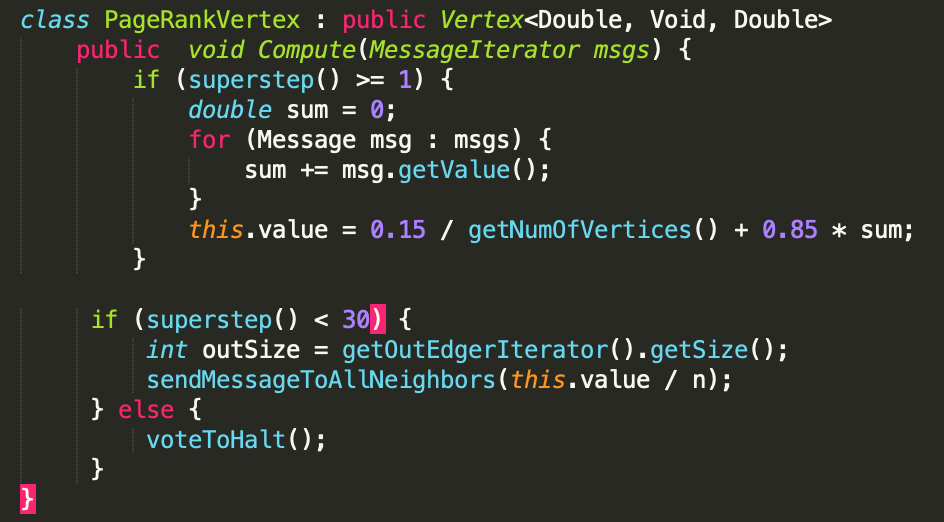
\includegraphics[width=0.4\textwidth]{img//pic5.png}
			%textwidth:正文宽度。双栏,则将两栏正文宽度相加。
		\caption{PageRank实现代码图}
		\label{pic5}
	\end{figure}
	
	从超级步1开始,每个顶点把发送过来的值都加到sum里。并且设置临时的PageRank值为0.15 / getNumOfVertices() + 0.85 * sum。到达超级步30后,不再发送信息,并且投票结束。实际运行中,PageRank算法可能会一直计算到收敛。
	
	\subsubsection{最短路径}
	为了简单明了,我们主要关注单源最短路径,即从一个顶点出发,到所有其他顶点的最短路径。
	\begin{figure}[htbp]
		\centering
		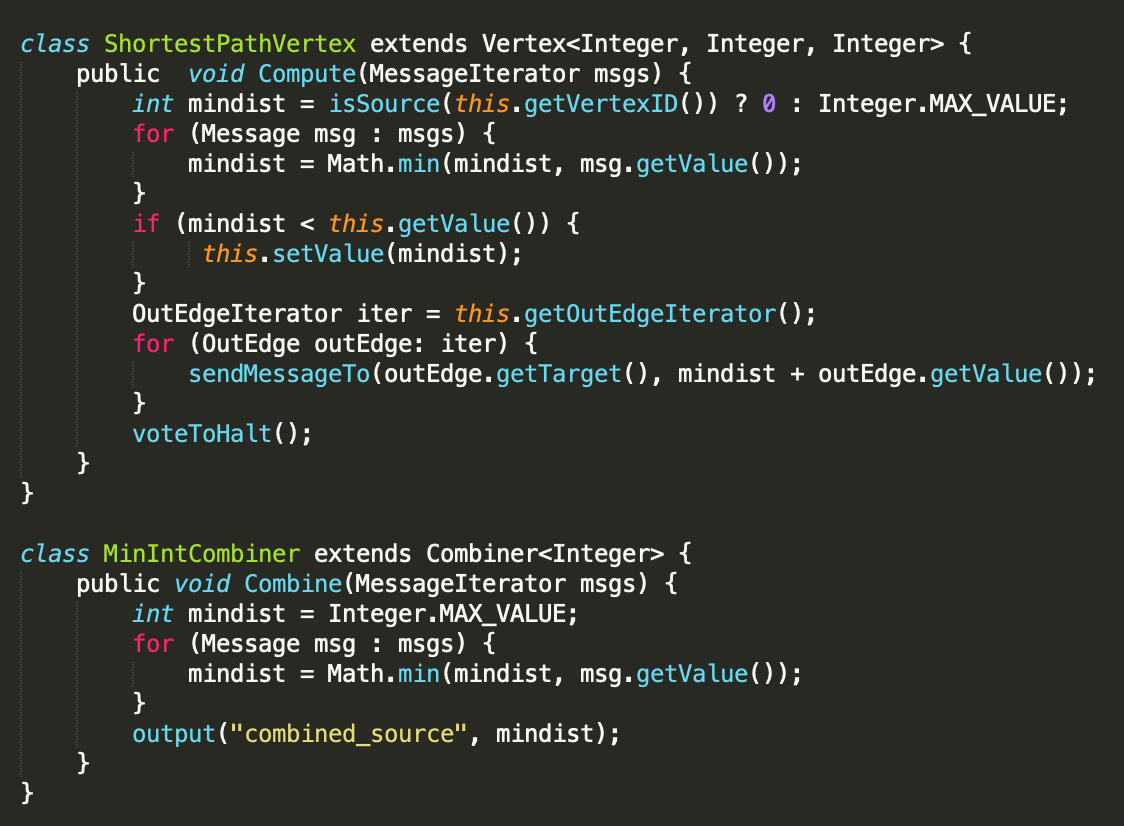
\includegraphics[width=0.4\textwidth]{img//pic6.png}
			%textwidth:正文宽度。双栏,则将两栏正文宽度相加。
		\caption{最短路径实现代码图}
		\label{pic6}
	\end{figure}
	
	在这个程序里,我们把每个顶点的初始距离都是$Integer.MAX\_VALUE$ 在每一超级步,每个顶点先接收从上游邻接顶点发过来的信息。用最小的值更新当前的值,然后更新它的下游邻接顶点。依次类推,此算法会在没有更新时结束。 \par
	本算法有一个Combiner来减少Woker之间传输的数据量。

\section{结束语}
	本文详细的介绍了Pregel这个大数据的一个分布式的编程框架,其关注于为用户提供一个自然的图计算API,并且隐藏分布式的一些细节,如信息传输和故障恢复。在概念上,它和MapReduce很相似,但是提供了更加自然的图API, 对图的迭代计算更高效。Pregel和Sawzall、Pig Latin、Dryad不同,因为Pregel隐藏了数据的分布细节。Pregel还有一点不一样,因为它实现了一个有状态的模型,它用一个长驻进程来实现计算、交换信息、修改本地状态,而不是用一个数据流模型。Pregel是为稀疏图设计的,主要是沿着边进行通信。尽管已经非常谨慎的支持高扇出、高扇入的信息流,但是当绝大部分顶点都和其他的大部分顶点进行通信时,性能会下降。一些类似的算法可以用Combiners、Aggregators、或者修改图来编写Pregel友好的算法。当然类似的计算对于任何的高度分布式的计算都困难。
	
%%end--------------------插入公式------------------------%%
% 这里文献较不规范 先不使用bib
%\printbibliography[title=参考文献]%打印参考文献
	%title:默认是英文的reference,用这个选参数改成中文
	
	\begin{thebibliography}{99}  
		\bibitem{ref1}Thomas Anderson, Susan Owicki, James Saxe, and Charles Thacker, High-Speed Switch Scheduling for Local-Area Networks. ACM Trans. Comp. Syst. 11(4), 1993, 319-352.		
		\bibitem{ref2}Luiz Barroso, Jerey Dean, and Urs Hoelzle, Web search for a planet: The Google Cluster Architecture. IEEE Micro 23(2), 2003, 22-28.  
		\bibitem{ref3}林子雨. 大数据技术原理与应用[M]. 北京:人民邮电出版社  
		\bibitem{ref4}蔡娇. 基于Pregel编程模型的图模式匹配方法[D].云南大学,2018.
		\bibitem{ref5}张骏雪. 面向大规模图数据处理的虚拟机管理系统研究与实现[D].东南大学,2016.
		\bibitem{ref6}李健,张晓琳,刘娇,高鹭,张换香.基于Pregel的分布式保护节点影响力匿名算法[J].计算机应用研究,2020,37(11):3428-3432.
	\end{thebibliography}


\end{document}
